\documentclass[11pt,a4paper,fleqn]{article}
\usepackage[UTF8]{ctex}
\usepackage[a4paper]{geometry}
\geometry{left=2.0cm,right=2.0cm,top=2.5cm,bottom=2.5cm}

\usepackage{amsmath,amsfonts,graphicx,amssymb,bm,amsthm}
\usepackage{mathrsfs}
\usepackage{algorithm,algorithmicx}
\usepackage{fancyhdr}
\usepackage{tikz}
\usetikzlibrary{intersections,through}
\usetikzlibrary{calc}
\usepackage{caption}
\usepackage{verbatim}
\usepackage{comment}

\renewcommand\thesection{Question \arabic{section}.}

\setlength{\headheight}{14pt}
\setlength{\parindent}{0 in}

\newtheorem{theorem}{Theorem}
\newtheorem{lemma}[theorem]{Lemma}
\newtheorem{proposition}[theorem]{Proposition}
\newtheorem{claim}[theorem]{Claim}
\newtheorem{corollary}[theorem]{Corollary}
\newtheorem{definition}[theorem]{Definition}

\newcommand\E{\mathbb{E}}
\newcommand{\hwid}{5}
\newcommand{\name}{梁昱桐}
\newcommand{\institute}{信息科学技术学院}
\newcommand{\id}{2100013116}
%\newcommand{\order}{324}

\usetikzlibrary{positioning}

\begin{document}

\pagestyle{fancy}
\lhead{Peking University}
\chead{}
\rhead{Principle of Economics, 2022 Fall}

\setlength{\parindent}{0pt}

\begin{center}
	{\LARGE \bf Principle of Economics Home Work \hwid}\\
	{\Large \name}\\
	{\Large \institute}\\
	{\Large \id}\\
	%{\Large \order}\\
\end{center}

\section{}
《遇见毕加索》毕加索真迹展将于10 月 1 日至 12 月 18 日在北京 798 遇见博物馆举行。假设该场地总共可容纳 35,000 人次。因此,发售的门票也固定在这一数量。由于看到了增加税收收入的机会,北京市政府决定向观众对每张门票征收 5 元的税收。假定征税前门票的单价是 500 元。

%\begin{comment}
\begin{itemize}

	\item[1)]请用供需模型画出征税前市场的均衡。

	\textbf{Solution:}

	\begin{center}
		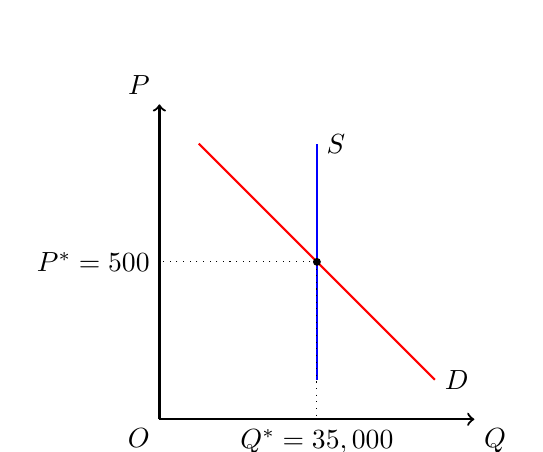
\begin{tikzpicture}
			%print x and y axis
			\coordinate[label=below left:{$O$}] (O)at(0,0);
			\coordinate[label=above left:{$P$}] (P)at(0,4);
			\coordinate[label=below right:{$Q$}] (Q)at(4,0);
			\draw[thick,->] (O)--(P);
			\draw[thick,->] (O)--(Q);
			%supply and demand curve
			\coordinate[label=right:{$S$}] (S) at(2,3.5);
			\coordinate[label=right:{$D$}] (D) at(3.5,0.5);
			\draw[name path=supply,domain=0.5:3.5,samples=100,smooth,variable=\x, blue,thick] plot({2},{\x});
			\draw[name path=demand,domain=0.5:3.5,samples=100,smooth,variable=\x, red,thick] plot({\x},{4-\x});
			%print vertical lines
			\path [name intersections={of=supply and demand}]
			coordinate (stable) at (intersection-1);
			\fill (stable) circle (.05);
			\coordinate[label=below:{$Q^*=35,000$}] (stable_q)at($(O)!(stable)!(Q)$);
			\coordinate[label=left:{$P^*=500$}] (stable_p)at($(O)!(stable)!(P)$);
			\draw[black,dotted] (stable)--(stable_q);
			\draw[black,dotted] (stable)--(stable_p);
		\end{tikzpicture}
	\end{center}

	\item[2)]请在图上画出征税后新的均衡。征税后市场上新的均衡价格是多少?

	\textbf{Solution:}
	
	\begin{center}
		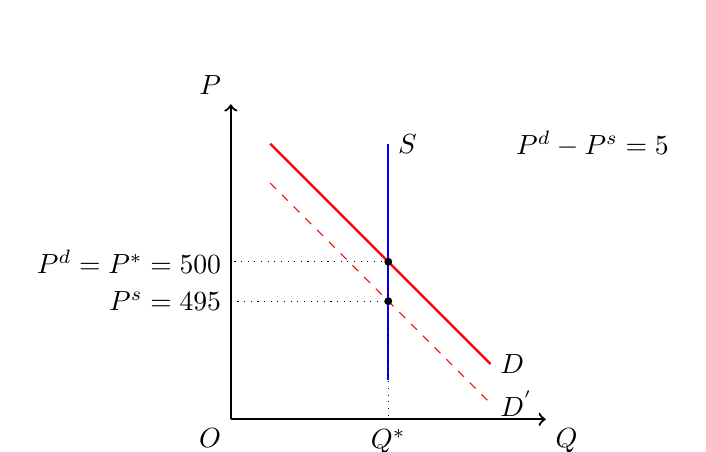
\begin{tikzpicture}
			%print x and y axis
			\coordinate[label=below left:{$O$}] (O)at(0,0);
			\coordinate[label=above left:{$P$}] (P)at(0,4);
			\coordinate[label=below right:{$Q$}] (Q)at(4,0);
			\draw[thick,->] (O)--(P);
			\draw[thick,->] (O)--(Q);
			%supply and demand curve
			\coordinate[label=right:{$S$}] (S) at(2,3.5);
			\coordinate[label=right:{$D$}] (D) at(3.3,0.7);
			\draw[name path=supply,domain=0.5:3.5,samples=100,smooth,variable=\x, blue,thick] plot({2},{\x});
			\draw[name path=demand,domain=0.5:3.3,samples=100,smooth,variable=\x, red,thick] plot({\x},{4-\x});
			%print vertical lines
			\path [name intersections={of=supply and demand}]
			coordinate (stable) at (intersection-1);
			\fill (stable) circle (.05);
			\coordinate[label=below:{$Q^*$}] (stable_q)at($(O)!(stable)!(Q)$);
			\coordinate[label=left:{$P^d=P^*=500$}] (stable_p)at($(O)!(stable)!(P)$);
			\draw[black,dotted] (stable)--(stable_q);
			\draw[black,dotted] (stable)--(stable_p);
			%supply elscity=0
			\coordinate[label=right:{$D^{'}$}] (D1) at(3.3,0.2);
			\draw[name path=demand1,domain=0.5:3.3,samples=100,smooth,variable=\x, red,dashed] plot({\x},{3.5-\x});
			\fill (2,1.5)circle(.05);
			\draw[dotted] (0,1.5)--(2,1.5);
			\coordinate[label=left:{$P^s=495$}] (stable1_p)at(0,1.5);
			%注释
			\coordinate[label=right:{$P^d-P^s=5$}] (NULL) at(3.5,3.5);
		\end{tikzpicture}
	\end{center}

	观众的均衡价格是500元,举办方能获得495元

	\item[3)]是举办方还是观众承担了更多的税收?请在图上画出观众和举办方各自的税收负担 (tax burden) ,并解释你的结论。

	\textbf{Solution:}
	
	\begin{center}
		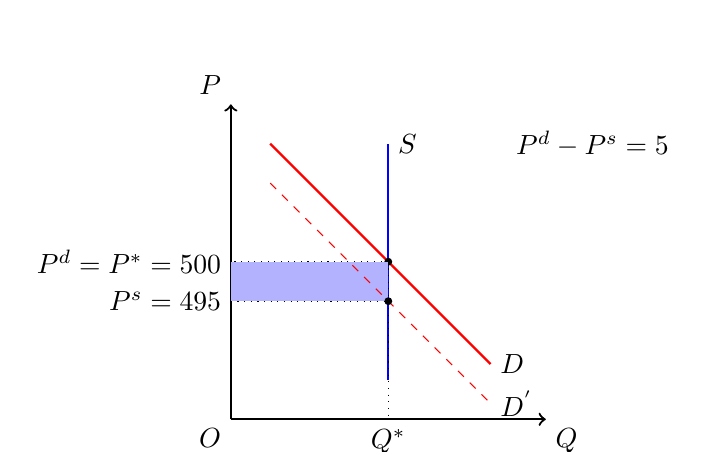
\begin{tikzpicture}
			%print x and y axis
			\coordinate[label=below left:{$O$}] (O)at(0,0);
			\coordinate[label=above left:{$P$}] (P)at(0,4);
			\coordinate[label=below right:{$Q$}] (Q)at(4,0);
			\draw[thick,->] (O)--(P);
			\draw[thick,->] (O)--(Q);
			%supply and demand curve
			\coordinate[label=right:{$S$}] (S) at(2,3.5);
			\coordinate[label=right:{$D$}] (D)at(3.3,0.7);
			\draw[name path=supply,domain=0.5:3.5,samples=100,smooth,variable=\x, blue,thick] plot({2},{\x});
			\draw[name path=demand,domain=0.5:3.3,samples=100,smooth,variable=\x, red,thick] plot({\x},{4-\x});
			%print vertical lines
			\path [name intersections={of=supply and demand}]
			coordinate (stable) at (intersection-1);
			\fill (stable) circle (.05);
			\coordinate[label=below:{$Q^*$}] (stable_q)at($(O)!(stable)!(Q)$);
			\coordinate[label=left:{$P^d=P^*=500$}] (stable_p)at($(O)!(stable)!(P)$);
			\draw[black,dotted] (stable)--(stable_q);
			\draw[black,dotted] (stable)--(stable_p);
			%coloured
			\fill[blue!30](0,1.5)--(2,1.5)--(2,2)--(0,2)--cycle;
			%supply elscity=0
			\coordinate[label=right:{$D^{'}$}] (D1) at(3.3,0.2);
			\draw[name path=demand1,domain=0.5:3.3,samples=100,smooth,variable=\x, red,dashed] plot({\x},{3.5-\x});
			\fill (2,1.5)circle(.05);
			\draw[dotted] (0,1.5)--(2,1.5);
			\coordinate[label=left:{$P^s=495$}] (stable1_p)at(0,1.5);
			%注释
			\coordinate[label=right:{$P^d-P^s=5$}] (NULL) at(3.5,3.5);

		\end{tikzpicture}
	\end{center}

	举办方承担了所有的税收,蓝色区域为举办方的税收负担,总共为 $35000\times (500-495)=175000$ 元

	因为举办方的门票发售量固定,不能离开市场,因此供给曲线弹性为0,从而举办方将承受所有的税收

	\item[4)]假定门票价格并不相同:有 10,000 张 VIP 早鸟票,每张门票价格 1,000 元; 另有 25,000 张普通票,每张门票价格 400 元。为了分析的简化,我们假定两个子市场是完全割裂的:购买早鸟票的观众不会因为价格的变动而考虑普通票;同理,购买普通票的观众不会因为价格的变动而考虑早鸟票。假定此时政府仍然决定对每张门票征收 5 元的税收,请计算此时观众和举办方各自的税收负担并与 3)中的结论做比较。

	\textbf{Solution:}
	
	仍然是举办方承担了所有的税收,税收与 3) 相同仍为175000元

\end{itemize}
%\end{comment}

\section{}
当北大校方决定增加对同学们就餐的补贴时(比如鸡腿饭变为 5 块!),校方补贴的金额会\_\_\_\_,同学们就餐时自我支付的金额最终会\_\_\_\_,北大学生和学校总体花在就餐上的金额最终会\_\_\_\_。

\begin{itemize}

	\item[A.]上升,下降,上升

	\item[B.]上升,可能上升或下降,可能上升或下降

	\item[C.]上升,可能上升或下降,上升

	\item[D.]可能上升或下降,可能上升或下降,可能上升或下降

\end{itemize}

\textbf{Solution:}C

\begin{center}
	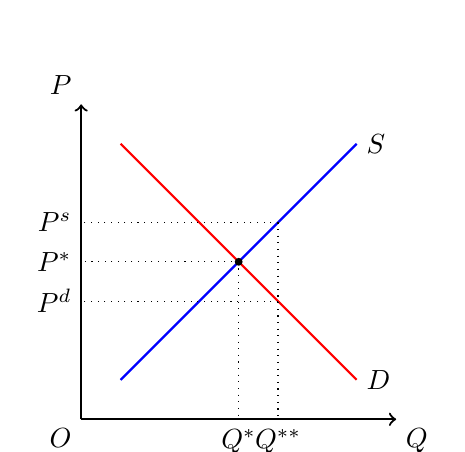
\begin{tikzpicture}
		%print x and y axis
		\coordinate[label=below left:{$O$}] (O)at(0,0);
		\coordinate[label=above left:{$P$}] (P)at(0,4);
		\coordinate[label=below right:{$Q$}] (Q)at(4,0);
		\draw[thick,->] (O)--(P);
		\draw[thick,->] (O)--(Q);
		%supply and demand curve
		\coordinate[label=right:{$S$}] (S) at(3.5,3.5);
		\coordinate[label=right:{$D$}](D) at(3.5,0.5);
		\draw[name path=supply,domain=0.5:3.5,samples=100,smooth,variable=\x, blue,thick] plot({\x},{\x});
		\draw[name path=demand,domain=0.5:3.5,samples=100,smooth,variable=\x, red,thick] plot({\x},{4-\x});
		\fill(2,2)circle(.05);
		%print vertical lines
		\draw[dotted](2,2)--(2,0);
		\draw[dotted](2,2)--(0,2);
		\draw[dotted](2.5,2.5)--(2.5,0);
		\draw[dotted](2.5,2.5)--(0,2.5);
		\draw[dotted](2.5,1.5)--(0,1.5);
		%print foot note
		\coordinate[label=below:{$Q^*$}](Q1) at(2,0);
		\coordinate[label=below:{$Q^{**}$}](Q2) at(2.5,0);
		\coordinate[label=left:{$P^*$}](P1) at(0,2);
		\coordinate[label=left:{$P^d$}](P2) at(0,1.5);
		\coordinate[label=left:{$P^s$}](P3) at(0,2.5);
	\end{tikzpicture}
\end{center}

校方补贴的金额变化量 $=(P^s-P^d)Q^{**}>0$

同学们就餐时自我支付的金额变化量 $=P^dQ^{**}-P^*Q^*$ 不能确定正负

北大学生和学校总体花在就餐上的金额变化量 $=P^sQ^{**}-P^*Q^*>0$

\section{}
开学以来你的电脑已经出了太多次故障,导致你想下一次电脑坏掉后不再维修,直接卖给中关村回收二手电脑的小贩2。为此,你准备提前研究一下二手电脑回收市场。假定中关村二手笔记本电脑回收市场的总供给曲线与总需求曲线如下:(注意此时供给与需求的主体,小贩为买方)

供给: $Q^s = 600+200P$

需求: $Q^d = 1800-400P$

其中, $Q^s$ 是二手电脑的供给曲线, $Q^d$ 是二手电脑的需求曲线。

\begin{itemize}

	\item[1)]请画出二手电脑的供给曲线与需求曲线(注意:价格在 $Y$ 轴上,所以供给曲线与需求曲线应该表示为函数  $P(Q)$ 的形式)。

	\textbf{Solution:}
	
	\begin{center}
		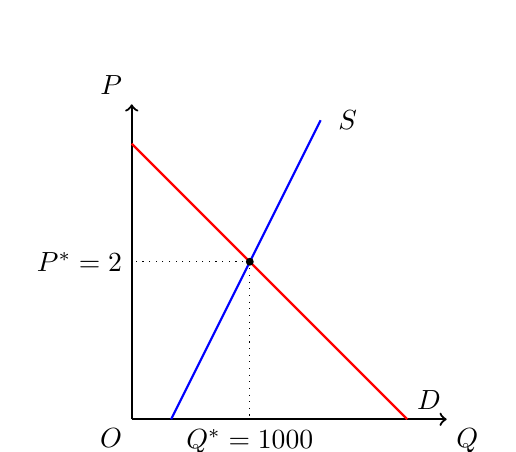
\begin{tikzpicture}
			%print x and y axis
			\coordinate[label=below left:{$O$}] (O)at(0,0);
			\coordinate[label=above left:{$P$}] (P)at(0,4);
			\coordinate[label=below right:{$Q$}] (Q)at(4,0);
			\draw[thick,->] (O)--(P);
			\draw[thick,->] (O)--(Q);
			%supply and demand curve
			\coordinate[label=right:{$S$}] (S) at(2.5,3.8);
			\coordinate[label=above right:{$D$}] (D) at(3.5,0);
			\draw[name path=supply,domain=0.5:2.4,samples=100,smooth,variable=\x, blue,thick] plot({\x},{-1+2*\x});
			\draw[name path=demand,domain=0:3.5,samples=100,smooth,variable=\x, red,thick] plot({\x},{3.5-\x});
			%print vertical lines
			\path [name intersections={of=supply and demand}]
			coordinate (stable) at (intersection-1);
			\fill (stable) circle (.05);
			\coordinate[label=below:{$Q^*=1000$}] (stable_q)at($(O)!(stable)!(Q)$);
			\coordinate[label=left:{$P^*=2$}] (stable_p)at($(O)!(stable)!(P)$);
			\draw[black,dotted] (stable)--(stable_q);
			\draw[black,dotted] (stable)--(stable_p);
			% %add tax
			% \path[name path=q_changed] (1.5,0)--(1.5,3);	
			% \path [name intersections={of=demand and q_changed}]
			%     coordinate (stable_d) at (intersection-1);
			% \path [name intersections={of=supply and q_changed}]
			%     coordinate (stable_s) at (intersection-1);
			% \coordinate[label=below:{$Q^{**}$}](stable_qq)at(1.5,0);			
			% \coordinate[label=left:{$P^d$}] (stable_d_p)at($(O)!(stable_d)!(P)$);
			% \coordinate[label=left:{$P^s$}] (stable_s_p)at($(O)!(stable_s)!(P)$);
			% \draw[black,dotted] (stable_d)--(1.5,0);
			% \draw[black,dotted] (stable_s)--(stable_s_p);
			% \draw[black,dotted] (stable_d)--(stable_d_p);
		\end{tikzpicture}
	\end{center}

	\item[2)]在均衡状态下,请计算二手电脑的均衡数量和均衡价格。此时,消费者剩余和生产者剩余分别是多少?

	\textbf{Solution:}
	
	$$
		\left\{
		\begin{aligned}
			Q^s &= 600+200P  \\
			Q^d &= 1800-400P \\
			Q^s &= Q^d
		\end{aligned}
		\right.
		\ \Longrightarrow\
		\left\{
		\begin{aligned}
			Q^s = Q^d & =1000 \\
			P         & = 2
		\end{aligned}
		\right.
	$$

	二手电脑的均衡数量为1000,均衡价格为2

	\item[3)]假设现在政府就每台被收购的二手电脑向卖方征税 $1.5$  单位价格,请回答以下问题:

	\begin{itemize}

		\item[a)]新的均衡价格和均衡数量是多少?
	
		\textbf{Solution:}
	
        $$
		\left\{
		\begin{aligned}
			Q &= 600+200P^s  \\
			Q &= 1800-400P^d \\
			P^s+1.5 &= P^d
		\end{aligned}
		\right.
		\ \Longrightarrow\
		\left\{
		\begin{aligned}
            Q&=800\\
			P^s  & =1 \\
			P^d   &=2.5 
		\end{aligned}
		\right.
	    $$

	    二手电脑的均衡数量为800,小贩收购的均衡价格为2.5,卖方能获得1
        
		\item[b)]税收负担更多的落在买方(小贩)还是卖方?为什么?

		\textbf{Solution:}
	
        税收更多落在卖方,因为在无税的均衡点处供给曲线斜率大,供给曲线比需求曲线弹性小,卖方会承受更多税收

		\item[c)]在新的均衡下,相比以前而言,小贩会花更多、更少还是一样的钱去收购二手电脑?

		\textbf{Solution:}
	
        $1000\times 2=800\times 2.5$ 因此花钱一样

		\item[d)]政府的税收收入是多少?

		\textbf{Solution:}
	
        $800\times 1.5=1200$
        
		\item[e)]卖方的收入会变多、变少还是不变?

		\textbf{Solution:}
	
        $1000\times 2>800\times 1$ 因此卖方的收入会变小

		\item[f)]现在的消费者剩余和生产者剩余变成了多少?

		\item[g)]请计算由于税收带来的无谓损失。

	\end{itemize}

	\item[4)]你认为对收购二手电脑的征税对于促进电子废弃物回收来说是好消息还是坏消息?

	\textbf{Solution:}
	
    坏消息,因为征税一定会使二手再利用的电子产品减少,从而电子废弃物增多

	\item[5)]如果征收 $100\%$ 的从价税,那么均衡价格和均衡数量是多少?(提示: $100\%$ 从价税的意思是,对于卖者收取的价格,政府对其征税额为现行价格的 $100\%$  .这和营业税是一样的道理。)

	\textbf{Solution:}
	
    $$
		\left\{
		\begin{aligned}
			Q &= 600+200P^s  \\
			Q &= 1800-400P^d \\
			P^s+P^s &= P^d
		\end{aligned}
		\right.
		\ \Longrightarrow\
		\left\{
		\begin{aligned}
            Q&=840\\
			P^s  & =1.2 \\
			P^d   &=2.4 
		\end{aligned}
		\right.
	    $$

        二手电脑的均衡数量为840,小贩收购的均衡价格为2.4,卖方能获得1.2
\end{itemize}

注:2)问以及 3)的 $f$ 和 $g$ 小问中涉及剩余和无谓损失的部分无需提交,等课上讲完福利分析后感兴趣的同学可自行练习。

\clearpage
\end{document}